

% Nastaven� �ablony FM TUL
% nastaveni prezentace
%\documentclass[draft]{beamer}
\documentclass[t]{beamer}

\usepackage[czech]{babel}

% FONTY

%\usepackage[cp1250]{inputenc} % pro win1250
\usepackage[T1]{fontenc}

\usepackage[utf8]{inputenc}
%\usepackage[IL2]{fontenc}

\usepackage{lmodern}

% XeLaTeX
%\usepackage{fontspec,lipsum}
%\defaultfontfeatures{Ligatures=TeX}
%\usepackage[small,sf,bf]{titlesec}
% 
%\setromanfont{Georgia}
%\setsansfont{Myriad Pro} %Tahoma}
%\setsansfont{Tahoma}
%\setsansfont{Arial}
%\setsansfont{Times New Roman}
%====

% bohu�el dal�� fonty nejsou pln� po�e�t�n�, tedy nejde bez obt��� kop�rovat z PDF

%\usepackage{times}
% \usepackage{avant}
% \usepackage{bookman}
% \usepackage{helvet}  %chyb� tu�n� �ez u strojov�ho p�sma
% \usepackage{newcent}
% \usepackage{palatino} 



%\usepackage[scaled]{uarial}
%\usepackage{helvet}


\usepackage{hyperref}

\mode<presentation>
{
  \definecolor{FM_TUL}{cmyk}{0,0.6,1,0}
  
  \useinnertheme{rectangles}
  
  % VN�J�� BAREVN� T�MA NADPIS�    
  \usecolortheme{whale}  
  
  % VNIT�N� BAREVN� T�MA V��T�, BLOK� ATD.  
  \usecolortheme{orchid}

  \setbeamercolor{titlelike}{parent=structure}
  \setbeamercolor{frametitle}{fg=black}
  \setbeamercolor{title}{fg=black}
  \setbeamercolor{item}{fg=FM_TUL} 
  \setbeamertemplate{navigation symbols}{} % potla�en� naviga�n�ch symbol�
  \setbeamercolor{block title}{fg=white,bg=FM_TUL} % p�edefinov�n� barvy z�kl. bloku
  \setbeamercolor{caption name}{fg=FM_TUL}
  
%  Nadpisy slid� tu�n� dokud nevy�e��m pou�it� font� tak, aby se dalo kop�rovat z pdf
%  \setbeamercolor{frametitle}{fg=FM_TUL}
  \setbeamertemplate{frametitle}
  {
    \textbf{\insertframetitle}
    \par
  }
  \setbeamercolor{bibliography entry author}{fg=black} % literatura �ern� a ne mod�e
  \setbeamercolor{bibliography entry title}{fg=black} % literatura �ern� a ne mod�e
  \setbeamercolor{bibliography entry journal}{fg=black} % literatura �ern� a ne mod�e
  \setbeamercolor{bibliography entry note}{fg=black} % literatura �ern� a ne mod�e
  
%Nefunguje  \setbeamercolor{tableofcontents}{fg=TUL_FM} % obsah TUL_FM a ne mod�e
}

%===============================================================================
% TITULN� STRANA
%===============================================================================
\setbeamertemplate{title page}{
\begin{flushleft}
   
\includegraphics[width=0.6\textwidth]{obr/logo-fm-cmyk-cz.pdf}
\end{flushleft} 
  %
\begin{center} 
  \setbeamercolor{postit}{fg=black,bg=FM_TUL}
%  \begin{beamercolorbox}[center,sep=2pt,wd=\textwidth,ht=3cm,dp=20pt]{postit}
 \begin{beamercolorbox}[center,sep=10pt,wd=\textwidth,ht=3.2cm,ignorebg]{postit}
            
      {\bf {\LARGE \inserttitle}}\\[16pt]
              
      \insertsubtitle
  \end{beamercolorbox}
%
  \vspace{10pt}
  {\bf \small \insertauthor {\color{FM_TUL} ~|} \insertdate}
%  \vspace{10pt}    
\end{center}
%
\vfill
\vskip0pt plus 1filll
{\color{FM_TUL} \hrule} 
%
\begin{center}
\vspace{-8pt}         
\TextTitulniStranaPodLinkou
\end{center}   
}
%===============================================================================
% Z�HLAV� KA�D�HO SLAJDU
%===============================================================================
\setbeamertemplate{headline}{
  \hspace{-3pt}
\includegraphics[width=0.3\textwidth]{obr/logo-fm-cmyk-cz.pdf}
}
%===============================================================================
\setbeamertemplate{footline}{

\includegraphics[width=\textwidth]{obr/FM_TUL_linka_piktogram_obd.pdf}

\vspace{-9.5pt}
~\hfill {\tiny\color{white} \insertframenumber\,/\,\inserttotalframenumber}\hspace{5pt}

\hspace{3pt} {\tiny \inserttitle {\color{FM_TUL} ~|} \insertdate }\hspace{3pt}
\vspace{3pt}
}
%===============================================================================
% �PRAVA BARVY TEXTU V OBSAHU 
%===============================================================================
\setbeamercolor{section in toc}{fg=black}
\setbeamercolor{subsection in toc}{fg=black}
\setbeamercolor{subsubsection in toc}{fg=black}
\setbeamercolor{button}{bg=FM_TUL}

%\definecolor{links}{HTML}{2A1B81}
\hypersetup{colorlinks,linkcolor=,urlcolor=FM_TUL}


\usepackage{palatino}
\usepackage{graphicx}
\usepackage{transparent}

\setbeamercovered{transparent=35}

\title[Pokročilý třídní jazykový slovníček]{Pokročilý třídní jazykový slovníček}
\subtitle{Diplomová práce}
\author[Bc.~Daniel~Maděra]{Bc.~Daniel~Maděra}
\institute[TUL]{Technická univerzita v Liberci}
\date{1.~února~2017}
\newcommand{\TextTitulniStranaPodLinkou}{\tiny
Studentská 2 {\color{FM_TUL} |} 461\,17 Liberec 2 {\color{FM_TUL} |} {daniel.madera@tul.cz} {\color{FM_TUL} |} 
\href{http://www.fm.tul.cz/}{www.fm.tul.cz}}

\renewcommand{\inserttotalframenumber}{\pageref{lastslide}}

\begin{document}
%\setbeamertemplate{caption}{\insertcaption}


\begin{frame}
    \titlepage
\end{frame}

\begin{frame}
    \frametitle{Obsah}
    \begin{itemize}
        \item problematika
        \item funkce aplikace
        \item grafické rozhraní
        \item architektura aplikace
        \item implementované algoritmy
        \item závěr
    \end{itemize}
\end{frame}


\begin{frame}[t]
    \frametitle{Problematika}
    \begin{itemize}[<+->]
        \item podnět od učitelů cizích jazyků na ZŠ
        \item učení slovní zásoby pomocí vlastního slovníčku
        \begin{itemize}
            \item chybí organizace
            \item bez adaptivního procvičování
            \item problematické opakování
        \end{itemize}
        \item aktuální výukové aplikace
        \begin{itemize}
            \item připravené pro samouky
            \item neumožňují se přizpůsobit aktuálně probírané slovní zásobě
            \item nelze sdílet slovní zásobu (učitel $\rightarrow$ žák)
        \end{itemize}
    \end{itemize}
\end{frame}

\begin{frame}[t]
    \frametitle{Funkce aplikace}
    \begin{itemize}[<+->]
        \item správa slov (učebnice, moduly, sdílení)
        \item hromadný import (automatizace, Google API)
        \item testovací sady
        \item adaptivní procvičování slov
        \item připomínání naučených slov
        \item motivace (generování slov, statistiky, pochvaly)
    \end{itemize}
\end{frame}

\begin{frame}[t]
    \frametitle{Grafické rozhraní - editace slov v učebnici}
    \begin{center}
        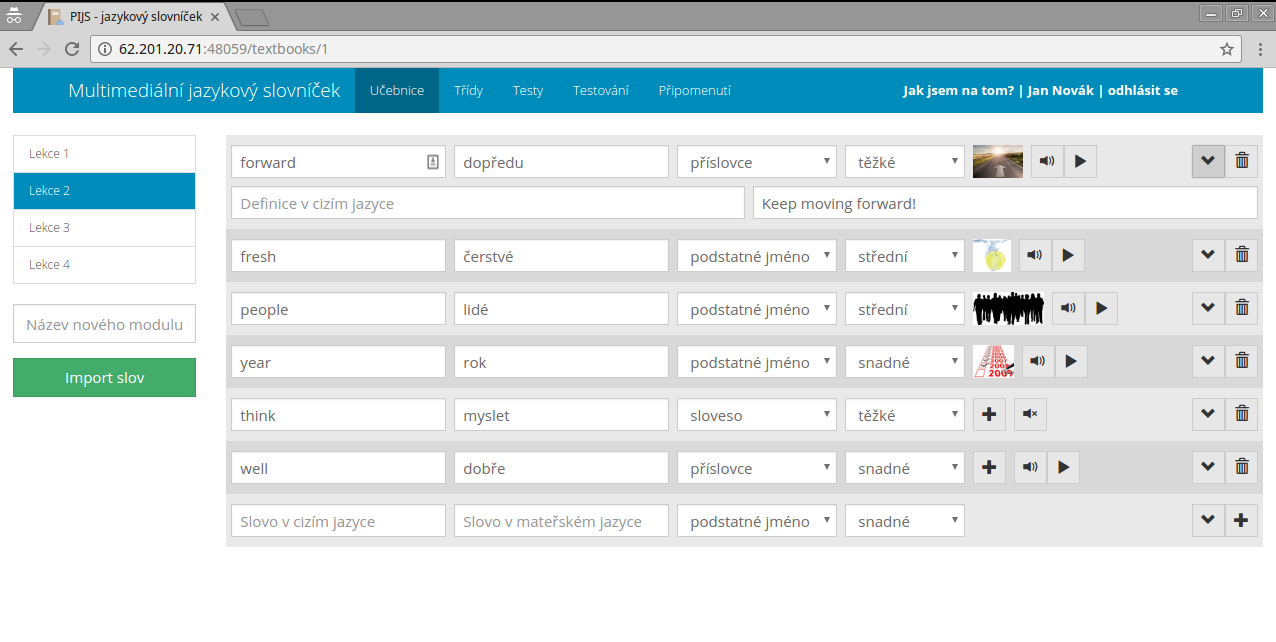
\includegraphics[width=\textwidth]{./img/gui-textbook-editor.png}\\
    \end{center}
\end{frame}

\begin{frame}[t]
    \frametitle{Grafické rozhraní - procvičování slov}
    \begin{center}
        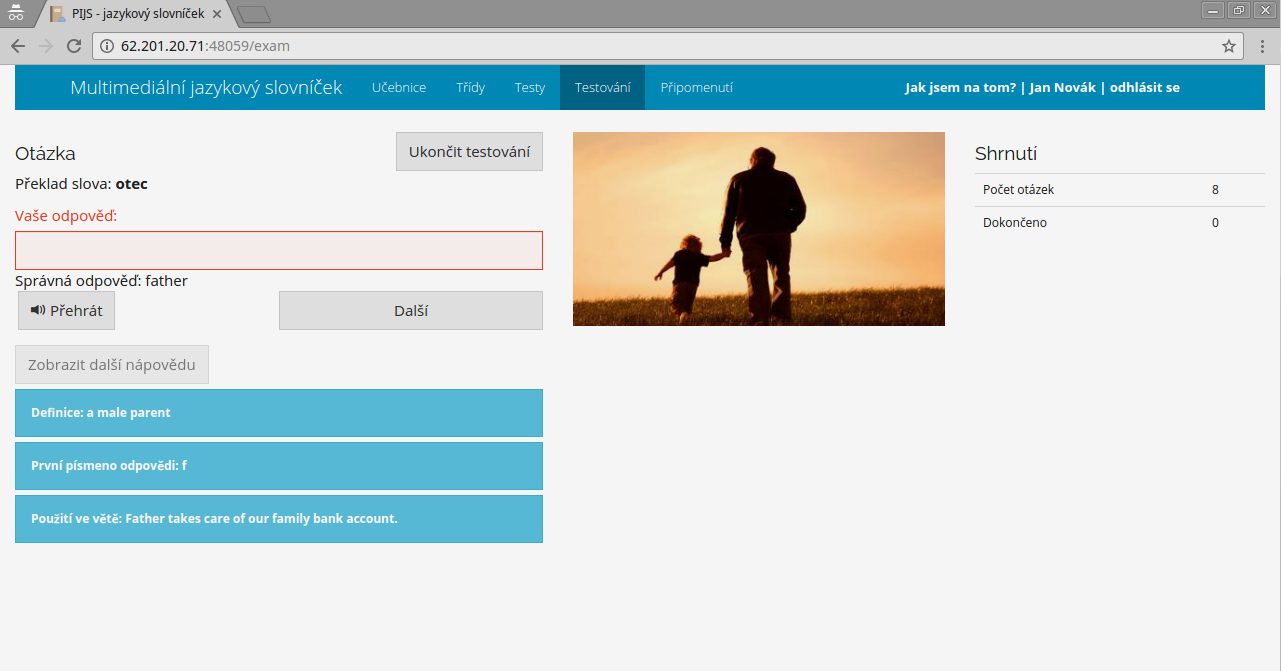
\includegraphics[width=\textwidth]{./img/gui-testing.png}\\
    \end{center}
\end{frame}

\begin{frame}[t]
    \frametitle{Architektura aplikace}
    \includegraphics[width=\textwidth]{./img/architecture.png}
\end{frame}

\begin{frame}[t]
    \frametitle{Generování slov pro procvičování}
    \begin{itemize}
        \item modifikovaný Leitnerův algoritmus
    \end{itemize}
    \only<1> {\includegraphics[width=\textwidth]{./img/words-gen-algorithm-0.png}}
    \only<2> {\includegraphics[width=\textwidth]{./img/words-gen-algorithm-1.png}}
    \only<3> {\includegraphics[width=\textwidth]{./img/words-gen-algorithm-2.png}}
    \only<4> {\includegraphics[width=\textwidth]{./img/words-gen-algorithm-3.png}}
    \only<5> {\includegraphics[width=\textwidth]{./img/words-gen-algorithm-4.png}}
\end{frame}

\begin{frame}[t]
    \frametitle{Připomínání slov}
    \begin{itemize}
        \item implementovaný algoritmus Supermemo
        \item metoda rozloženého opakování
        \item intervaly: 1d, 3d, 13d, 24d, 1m, 7m 
    \end{itemize}
    \begin{center}
        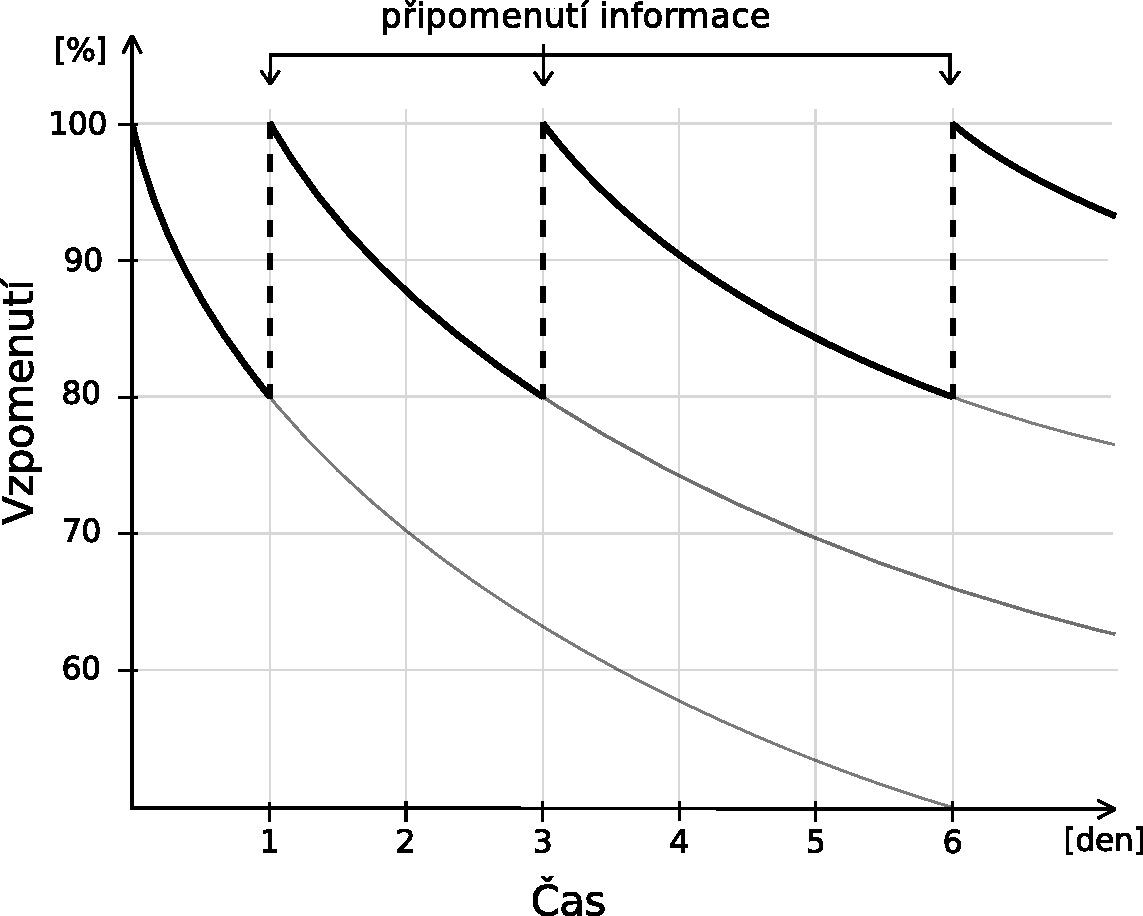
\includegraphics[width=6.5cm]{./img/forgetting-curve.pdf}\\
    \end{center}
\end{frame}

\begin{frame}[t]
    \frametitle{Závěr}
    \begin{itemize}[<+->]
        \item rešerše existujících aplikací 
        \item navržena a implementována aplikace
        \item správa a import slovíček, tříd a testovacích sad
        \item automatické získání další interpretační formy slova (zvuk, obrázek)
        \item motivující a adaptivní procvičování
        \item připomínání slovíček v efektivních intervalech
        \item testování aplikace externími uživateli
    \end{itemize}
\end{frame}


\begin{frame}
\begin{center}
\label{lastslide}
\huge Děkuji za pozornost.
\end{center}
\end{frame}

\begin{frame}[noframenumbering]
    \frametitle{Existují další možnosti stanovení obtížnosti slovíček? Jakým způsobem by změna metody ovlivnila aplikaci?}

    \begin{itemize}
        \item aktuálně obtížnost slov - vážený průměr
        \begin{itemize}
            \item délka slov, podobnost s výrazem v mateřském jazyce, výskyt přehlasování a dvojitých písmen
            \item $\rightarrow$ lze editovat jeho parametry
        \end{itemize}
        \item další možnosti
        \begin{itemize}
            \item fonetická podobnost
            \item hodnota častého výskytu (most frequent words)
            \item statisticky
        \end{itemize}
        \item není stěžejní, je později přepsáno uživatelskou obtížností
        \item ovlivnila by motivaci žáků (nutných správných opakování pro dokončení slova)
    \end{itemize}
\end{frame}

\begin{frame}[noframenumbering]
    \frametitle{Jaký může být důsledek toho, že není použito API dle REST ale vlastní řešení?}
    \begin{itemize}
        \item ztížené programování dalšího klienta 
        \item nutné nastudování přesné struktury API 
        \begin{itemize}
            \item popisuje RAML soubor (RESTful API Modeling Language)
        \end{itemize}
    \end{itemize}
\end{frame}

\begin{frame}[noframenumbering]
\begin{center}
    \frametitle{Pro práci byla zvolena integrace se službami Google. Byly zvažovány i další možnosti, např. integrace výkladového slovníku apod.?}

    \begin{itemize}
        \item integrace výkladového slovníku a překladu slova
        \begin{itemize}
            \item zodpovědnost ponechána na vyučujícím
            \item přizpůsobí definici slov úrovni cílených žáků
            \item různé významy by mohly být pro žáky matoucí
        \end{itemize}
        \item integrace rozpoznání řeči
        \begin{itemize}
            \item kontrola správné výslovnosti
            \item nutná HW podpora mikrofonu
            \item možnost využít služeb (placené)
            \item vlastní implementace - další možné rozšíření (náročné)
        \end{itemize}
    \end{itemize}
    % pouze k doplnění ke slovu je možné uložit i definici a použití ve větě
    % ano byla zvážena možnost výkladového slovníku, ale nakonec se od této možnosti distancovalo, jelikož každý vyučující může slovo definovat žákům v hodinách po svém a mohlo by dojít k žáci by potom cizím definicím nemuseli porozumět
    % zároveň vyučující přizpůsobí definici slov dle vlastního uvážení - bude využívat takovou slovní zásobu, která odpovídá úrovni žáků
    % další možností, která byla v úvaze, bylo získávat překlad slova, ale znovu by vyučující mohli narážet na problém, že významy slov zcela nekorespondují s těmi, které sdělovali dětem - například více významová slova

\end{center}
\end{frame}

\end{document}
